% =====================================================================
%  Chapter 2 — The Artifact
% =====================================================================

\chapter{The Artifact: 175,187 Files}
\label{ch:artifact}

Chapter~1 reported what the claim says. This chapter reports what was
submitted, because the two are not the same thing and the difference is where
the whole question lives.

\section{Acquisition}

The remark's first footnote gives the distribution point: a fourteen-part
tarball at \texttt{alpo.ge/lean.tar.gz.part01} through \texttt{.part14}. All
fourteen parts were downloaded for this book, concatenated, and extracted. The
result is 239{,}275{,}554 bytes of compressed archive expanding to 175{,}187
Lean source files occupying approximately one gigabyte.

The submission pins two things, and the pins matter:

\begin{itemize}
\item The toolchain: \texttt{leanprover/lean4:v4.33.1}, read from the
repository's \texttt{lean-toolchain} file.
\item The library: Mathlib at revision
\texttt{0df444a360eaa60ab8c11dca51a86af692955474}, read from the repository's
\texttt{lakefile.toml}. This revision was confirmed locally after a checkout:
\texttt{git rev-parse HEAD} in the fetched Mathlib returns exactly that string.
\end{itemize}

Pinning the library is the right practice, and it makes the artifact
reproducible in principle. It also means that a future audit is a statement
about \emph{that} revision of Mathlib and not about whatever Mathlib has
become by the time the audit is done.

\section{The shape of the development}

The tree is not one program but ten libraries, each a separate Lean package
within the Lake workspace. The census below was computed for this book by
counting files on disk.

\begin{figure}[H]
\centering
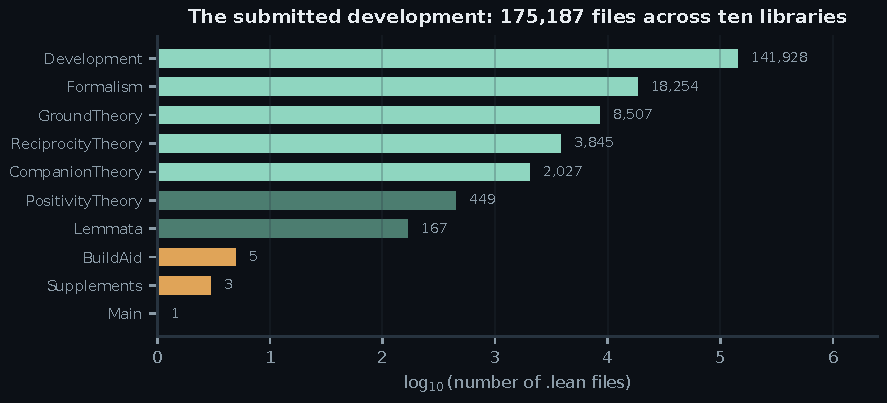
\includegraphics[width=\textwidth]{../figures/fig_library.pdf}
\caption{The submitted development by library, on a logarithmic scale. The
concentration is extreme: one library, \texttt{Development}, holds 81 per cent
of the files. Counts were computed locally from the extracted submission.}
\label{fig:library}
\end{figure}

\tabref{tab:census} gives the numbers, and one structural observation.

\begin{table}[H]
\centering
\caption{Library census of the submitted development.}
\label{tab:census}
\begin{tabular}{@{}lrl@{}}
\toprule
\textbf{Library} & \textbf{Files} & \textbf{Share} \\
\midrule
\texttt{Development}      & 141{,}928 & 81.1\% \\
\texttt{Formalism}        & 18{,}254  & 10.4\% \\
\texttt{GroundTheory}     & 8{,}507   & 4.9\% \\
\texttt{ReciprocityTheory}& 3{,}845   & 2.2\% \\
\texttt{CompanionTheory}  & 2{,}027   & 1.2\% \\
\texttt{PositivityTheory} & 449       & 0.3\% \\
\texttt{Lemmata}          & 167       & 0.1\% \\
\texttt{BuildAid}         & 5         & $<0.01\%$ \\
\texttt{Supplements}      & 3         & $<0.01\%$ \\
\texttt{Main}             & 1         & $<0.01\%$ \\
\midrule
\textbf{Total}            & \textbf{175{,}187} & 100\% \\
\bottomrule
\end{tabular}
\end{table}

The library names are not arbitrary. \texttt{Formalism} holds the abstract
scaffolding --- the general machinery for periods, integrals, lattices, mass
formulas and reciprocity. \texttt{GroundTheory} holds the geometric
foundations. \texttt{ReciprocityTheory} holds the reciprocity and
automorphic-form theory. \texttt{PositivityTheory} holds the positivity and
estimate arguments, which is where the analytic heavy lifting lives.
\texttt{Development} holds the specific theorems.

This is not the shape of a generated proof attempt. It is the shape of a
programme of work: a general library built alongside a specific one, with
shared abstractions factored out as they were discovered.

\section{What the artifact claims}

The entire public surface of the submission is \texttt{src/Main.lean}\idx{Lean development:structure of}, which
is 433 bytes long and reads in full:

\begin{seamnote}{\texttt{src/Main.lean}}
\begin{verbatim}
import Statements
import Supplements.Kernels.MainTheoremsAll

theorem riemannHypothesis : RiemannHypothesis := rhOfAll

theorem riemannZeta_eq_zero_re : RiemannZetaZerosOnLine := rhOfAll

theorem LFunction_ne_zero_of_half_lt_re :
    DirichletLNonvanishingRightOfHalf := allChi

theorem LFunction_eq_zero_re : DirichletLZerosOnLine := claimAll.2.1

theorem LFunction_eq_zero_re_of_isPrimitive :
    PrimitiveDirichletLZerosOnLine := critAll
\end{verbatim}
\end{seamnote}

Six theorems, all discharging into named constants. Note what is \emph{not}
here: no hypotheses, no parameters, no conditional statements, no ``assuming
the following'', no \texttt{sorry}. The top-level artifact asserts six
unconditional theorems.

The statements themselves live in \texttt{src/Statements.lean}\idx{Lean development:statements}, 783 bytes, and
are equally short. This is the part that most deserves a careful reading,
because a formalisation claim can always be true in the trivial sense that the
statement was weakened. Here it is not.

\begin{seamnote}{\texttt{src/Statements.lean} (the two statements that matter)}
\begin{verbatim}
def RiemannZetaZerosOnLine : Prop :=
  forall s : Complex, riemannZeta s = 0 ->
    (not exists n : Nat, s = -2 * ((n : Complex) + 1)) ->
    s != 1 -> s.re = 1 / 2

def DirichletLNonvanishingRightOfHalf : Prop :=
  forall (N : Nat) [NeZero N] (chi : DirichletCharacter Complex N) (s : Complex),
    1 / 2 < s.re -> (chi != 1 or s != 1) ->
    DirichletCharacter.LFunction chi s != 0
\end{verbatim}
\end{seamnote}

These are the standard formulations, faithfully transcribed. The first says:
every zero of the Riemann zeta function other than the trivial ones
($s = -2, -4, -6, \dots$) and other than the pole at $s = 1$ has real part
exactly $\tfrac12$. That \emph{is} the Riemann hypothesis. The second says: no
Dirichlet $L$-function has a zero strictly to the right of the critical line,
with the single exception of the principal character's pole at $s = 1$. That is
the standard equivalent non-vanishing form, and by the same token it is the
generalised Riemann hypothesis for Dirichlet $L$-functions.

Two things follow, and they are the first two results of the audit.

\begin{keytakeaways}

\item \textbf{The statement is the real statement.} The submission does not
weaken the target. It proves Mathlib's own \texttt{RiemannHypothesis}, and
Mathlib's own definition is the one written above.
\item \textbf{The submission is not conditional.} There are no hypotheses in
\texttt{Main.lean} and no hypotheses in \texttt{Statements.lean}.
\end{keytakeaways}

\section{The mirror, and one line that matters}

A third party mirrored the archive on GitHub the same day, as
\texttt{CocoSgt/riemann-hypothesis-lean}\idx{CocoSgt mirror}, with a description that reads:
``Mirror of Levent Alpöge's Lean proof of the Riemann Hypothesis (with Claude).
All credit to Levent Alpöge. Source: alpo.ge''. The mirror also records a
static scan of the archive and a set of recommended verification steps.

One line of that README has been quoted widely, including in newspaper
coverage, and it needs its date attached:

\begin{quote}
\small
``\textbf{Status.} As of mirroring (2026-11-20), no independent build or review\idx{status line, dated}
of this code has been published. Treat it as a claimed proof until it has been
compiled and checked.''
\end{quote}

That line was true when it was written, on the morning of 20 November. By noon
that day, Chapter~10 shows, two independent compilations had been completed.
The line should therefore be read as a dated status, not a current one, and any
book that repeats it without the date is misleading its readers.

The sentence's second clause --- \emph{``until it has been compiled and
checked''} --- is the more durable part, and it distinguishes two activities
that are constantly conflated. Compilation has happened. Checking has not.

\section{What is in the archive: the audit's first results}

The three mechanical facts that can be established about the artifact without
compiling it are these.

\begin{enumerate}
\item \textbf{There are no axioms.}\idx{axioms (Lean)} A full-tree scan of all 175{,}187 files
found zero declarations matching \texttt{axiom}. This includes the file names
the artifact's own library structure would suggest: the abstract theorems live
in \texttt{Formalism} and \texttt{GroundTheory}, and neither contains a single
axiom.
\item \textbf{There are no admitted gaps.} The same scan found zero
occurrences of \texttt{sorry}. The mirror's independent scan reports the same
and adds \texttt{admit} 0, \texttt{native\_decide} 0, and
\texttt{unsafe}/\texttt{implemented\_by}/\texttt{@[extern]} 0.
\item \textbf{The headline statement comes from outside the artifact.} The
mirror notes, correctly, that \texttt{RiemannHypothesis} is Mathlib's own
definition, from
\texttt{Mathlib/NumberTheory/LSeries/RiemannZeta.lean} at line 185 at the
pinned commit. The submission is not asserting a private definition of the
hypothesis; it is proving the community's.
\end{enumerate}

It would be easy, and wrong, to stop here. Zero axioms and zero \texttt{sorry}
are strong and necessary conditions, and they are not sufficient. A theorem
whose \emph{statement} quietly contains the hard content --- an unproved
hypothesis re-packaged as a lemma, with a classical name --- will show up
cleanly in both scans. The reason is structural: the scan looks for a marker
inside the proof, and the failure mode lives in the statement.

Chapter~7 and Chapter~8 are about that failure mode, and about how far a
reading of the source gets without running the compiler.

\section{One more structural observation}

The artifact's own scan reports, and this book's scan confirms, that
\texttt{set\_option maxHeartbeats 0} appears in four files, that custom
\texttt{macro}/\texttt{elab}/\texttt{syntax} declarations appear in 22 files,
and that \texttt{addDecl} appears in one file.

None of these is evidence of anything, in either direction, and this book
treats them that way. They are worth recording for one reason only: they are
the places where a future auditor should look first, because they are the
places where the \emph{elaborator} --- as opposed to the kernel --- is doing
something unusual. A custom macro that expands a proof obligation into
something trivial is the classic way to make a proof look complete without
making it so. Whether that happens here is unknown; the check is cheap, and
Chapter~14 includes it.

\begin{mythbox}{Three claims about this artifact that should not be made}
\begin{itemize}
\item \emph{``It is obviously a fake because no AI could do this.''} The
author's own prior work --- the two-thirds theorem of Chapter~11 --- is a
genuine, formally verified result using the same method family, and it was
reproduced independently by a third party. The method is not a fantasy.
\item \emph{``Zero axioms and zero sorry means it is proved.''} It means the
\emph{formal} layer is clean. Whether the formal statements mean what the
author says they mean is a separate question, and it is the question nobody has
yet answered. See Chapter~6.
\item \emph{``It compiles, therefore the Riemann Hypothesis is proved.''} It
compiles. What has been compiled is a development whose hardest inputs have
never been read by anyone outside its author. A proof assistant will happily
check a proof of a statement that is weaker than you think, and it will do so
without complaint.
\end{itemize}
\end{mythbox}

\vspace{8pt}
\noindent{\small\color{txtdim}\sffamily
The source tree examined in this book was extracted locally to
\texttt{/workspace/rr/src/lean/} and all file paths quoted in Chapters~7 to~9
are relative to that root. The scans reported in Chapter~9 were run over the
complete extraction, not a sample.\par}
